\section{Polyhedral sets in standard form}

In the context of linear programming problems, we will often consider problems written in the so-called \emph{standard form}. The standard form can be understood as posing the linear programming problem as an underdetermined system of equations (that is, with fewer equations than variables). Then, we will work on selecting a subset of the variables to be set to zero so that the number of remaining variables is the same as that of equations, making the system solvable. 

A key point in this chapter will be devising how we relate this process of selecting variables with that of selecting a subset of active constraints (forming a vertex, as we have seen in the previous chapter) that will eventually lead to an optimal solution. 


\subsection{The standard form of linear programming problems}

First, let us formally define the notion of a standard-form polyhedral set. Let $A$ is a $m \times n$ matrix and $b \in \reals^m$. The \emph{standard form} polyhedral set $P$ is given by 
%
\begin{equation*}
	P = \braces{x \in \reals^n : Ax = b, x \geq 0}.		
\end{equation*}
%
We assume that the $m$ equality constraints are linearly independent, i.e., $A$ is full (row) rank ($m \leq n$). We know that a basic solution can be obtained from a collection of $n$ active constraints since the problem is defined in $\reals^n$. 

One important point is that \emph{any} linear programming problem can be represented in the standard form. This is achieved utilising nonnegative \emph{slack variables}. Thus, a feasibility set that is, say, originally represented as
%
\begin{equation*}
	P = \braces{x \in \reals^n : A_1 x \le b_1, A_2x \ge b_2, x \ge 0}
\end{equation*}
%
can be equivalently represented as a standard-form polyhedral set. For that, it must be modified to consider slack variables $s_1 \ge 0$ and $s_2 \geq 0$ such that
%
\begin{equation*}
	P = \braces{(x, s_1, s_2) \in \reals^{(n + |b_1| + |b_2|)} : A_1 x + s_1 = b_1, A_2x - s_2 = b_2, (x, s_1, s_2) \ge 0},
\end{equation*}
%
where $|u|$ represents the cardinality of the vector $u$. Another transformation that may be required consists of imposing the condition $x \ge 0$. Let us assume that a polyhedral set $P$ was such that (notice the absent nonnegativity condition)
%
\begin{equation*}
	P = \braces{x \in \reals^n : Ax = b}.		
\end{equation*}
%
It is a requirement for standard-form linear programs to have all variables to be assumed nonnegative. To achieve that in this case, we can simply include two auxiliary variables, say $x^+$ and $x^-$, with the same dimension as $x$, and reformulate $P$ as
 %
\begin{equation*}
	P = \braces{x^+,x^- \in \reals^n : A(x^+ - x^-) = b, x^+, x^- \ge 0}.		
\end{equation*}
%

These transformations, as we will see, will be required for employing the simplex method to solve linear programming problems with inequality constraints and, inevitably, will always render standard form linear programming problems with more variables than constraints, or $m < n$.

The standard-form polyhedral set $P$ always has, by definition, $m$ active constraints because of its equality constraints. To reach the total of $n$ active constraints, $n-m$ of the remaining constraints $x_i \ge 0$, $i =1,\dots, n$, must be activated, and this is achieved by selecting $n-m$ of those to be set as $x_i = 0$. These $n$ active constraints (the original $m$ plus the $n-m$ variables set to zero) form a basic solution, as we seen in the last chapter. If it happens that the $m$ equalities can still be satisfied while the constraints $x_i \ge 0$, $i =1,\dots, n$, are satisfied, then we have a basic feasible solution (BFS). Theorem \ref{p1c3:thm:LI_and_bases} summarises this process, guaranteeing that the setting of $n-m$ variables to zero will render a basic solution.

\begin{theorem}[Linear independence and basic solutions] \label{p1c3:thm:LI_and_bases}
	Consider the constraints $Ax = b$ and $x \geq 0$, and assume that $A$ has $m$ linearly independent (LI) rows $M = \braces{1,\dots,m}$. A vector $\overline{x} \in \reals^n$ is a basic solution if and only if we have that $A \overline{x} = b$ and there exists indices $B(1), \dots, B(m)$ such that
	\begin{enumerate}
		\item[(1)] The columns $A_{B(1)}, \dots, A_{B(m)}$ of $A$ are LI
		\item[(2)] If $j \neq B(1), \dots, B(m)$, then $\overline{x}_j = 0$.
	\end{enumerate} 
\end{theorem}

\begin{proof}
	Assume that (1) and (2) are satisfied. Then the active constraints $\overline{x}_j = 0$ for $j \notin \braces{B(1), \dots, B(m)}$ and $Ax = b$ imply that
%	
	\begin{equation*}
		\sum_{i=1}^m A_{B(i)}\overline{x}_{B(i)} = \sum_{j=1}^n A_j\overline{x}_j = A\overline{x} = b.
	\end{equation*}
%
	Since the columns $\braces{A_{B(i)}}_{i \in M}$ are LI, $\braces{\overline{x}_{B(i)}}_{i \in M}$ are uniquely determined and thus $A\overline{x} = b$ has a unique solution, implying that $\overline{x}$ is a basic solution (cf. Theorem \ref{p1c2:thm:BFS_vertex_extreme_point}).
	
	Conversely, assume that $\overline{x}$ is a basic solution. Let $\overline{x}_{B(1)}, \dots, \overline{x}_{B(k)}$ be the nonzero components of $\overline{x}$. Thus, the system 
%	
		\begin{equation*}
			\sum_{i=1}^n A_i\overline{x}_i = b \text{ and } \braces{\overline{x}_i = 0}_{i \notin \braces{B(1), \dots, B(k)}}
		\end{equation*}
%
	has a unique solution, and so does $\sum_{i=1}^k A_{B(i)}\overline{x}_{B(i)} = b$, implying that the columns $A_{B(1)}, \dots, A_{B(k)}$ are LI. Otherwise, there would be scalars $\lambda_1,\dots, \lambda_k$, not all zeros, for which $\sum_{i=1}^k A_{B(i)}\lambda_i = 0$; this would imply that $\sum_{i=1}^k A_{B(i)}(\overline{x}_{B(i)} + \lambda_i) =b$, contradicting the uniqueness of $\overline{x}$.
	Since $A_{B(1)}, \dots, A_{B(k)}$ are LI, $k \leq m$. Also, since $A$ has $m$ LI rows, it must have $m$ LI columns spanning $\reals^m$. Using Theorem \ref{p1c2:thm:LI_and_bases}, we can obtain $m-k$ additional columns $A_{B(k+1)}, \dots, A_{B(m)}$ so that $A_{B(1)}, \dots, A_{B(m)}$ are LI. 
	
	Finally, since $k \leq m $, $\braces{\overline{x}_j = 0}_{i \notin \braces{B(1), \dots, B(m)}} \subset  \braces{\overline{x}_j = 0}_{i \notin \braces{B(1), \dots, B(k)}}$, satisfying (1) and (2). \qedhere 		
\end{proof}	

This proof highlights an important aspect in the process of generating basic solutions. Notice that once we set $n-m$ variables to be zero, the system of equations forming $P$ becomes uniquely determined, i.e., 
%
\begin{equation*}
	\sum_{i=1}^m A_{B(i)}\overline{x}_{B(i)} = \sum_{j=1}^n A_j\overline{x}_j = A\overline{x} = b.
\end{equation*}	
%


\subsection{Forming bases for standard-form linear programming problems}

Theorem \ref{p1c3:thm:LI_and_bases} provides us with a way to develop a simple procedure to generate all basic solutions of a linear programming problem in standard form.

\begin{enumerate}
	\item Choose $m$ LI columns $A_{B(1)}, \dots, A_{B(m)}$;
	\item Let $x_j = 0$ for all $j \notin \braces{B(1), \dots, B(m)}$;
	\item Solve the system $Ax = b$ to obtain $x_{B(1)}, \dots, x_{B(m)}$.
\end{enumerate}

You might have noticed that in the proof of Theorem \ref{p1c3:thm:LI_and_bases}, the focus shifted to the columns of $A$ rather than its rows. The reason for that is because, when we think of solving the system $Ax = b$, what we are truly doing is finding a vector $x$ representing the linear combination of the columns of $A$ that yield the vector $b$. This creates an association between the columns of $A$ and the components of $x$ (i.e., the variables). Notice, however that the columns of $A$ are not \emph{the} variables per se, as they have dimension $m$ (while $x \in \reals^n$). 

One important interpretation for Theorem \ref{p1c3:thm:LI_and_bases} is that we will form bases for the column space of $A$ by choosing $m$ components to be nonzero in a vector of dimension $n$. Since $m < n$ by definition, $A$ can only have rank $\rank(A) = \min{m,n} = m$, which happens to be the size of both the row space of $A$ (as the rows are assumed LI). This, in turn, means that both the column and the row spaces have dimension $m$. Thus, these bases are bases for the column space of $A$. Finally, finding the vector $x$ is the same as finding how the vector $b$ can be expressed as a linear combination of that basis. Notice that this is always possible when the basis spans $\reals^m$ (as we have $m$ LI column vectors) and $b \in \reals^m$.

You will notice that from here onwards, we will implicitly refer to the columns of $A$ as variables (although we actually mean the weight associated with that column, represented by the respective component in the variable $x$). Then, when we say that we are setting some ($n-m$) of the variables to be zero, it means that we are ignoring the respective columns of $A$ (the mapping between variables and columns being their indices: $x_1$ referring to the first column, $x_2$ to the second, and so forth), while using the remainder to form a (unique) combination that yields the vector $b$, being the weights of this combination precisely the solution $x$, which in turn represent the coordinates in $\reals^n$ of the vertex formed by the $n$ ($m$ equality constraints plus $n-m$ variables set to zero) active constraints.   

As we will see, this procedure will be at the core of the simplex method. Since we will often refer to elements associated with this procedure, it will be useful to define some nomenclature.

We say that $B = \braces{A_{B(i)}}_{i \in I_B}$ is a \emph{basis} (or, perhaps more precisely, a basic matrix) with basic indices $I_B = \braces{B(1), \dots, B(m)}$. Consequently, we say that the variables $x_j$, for $x_j$, for $j \in I_B$, are \emph{basic variables}. Somewhat analogously, we say that the variables chosen to be set to zero are the \emph{nonbasic variables} $x_j$, for $j \in I_N$, where $I_N = J \setminus I_B$, with $J = \braces{1, \dots, n}$ being the indices of all variables (and all columns of $A$).
 
 Notice that the basic matrix $B$ is invertible, since its columns are LI (c.f. Theorem \ref{p1c2:thm:LI_and_bases}). For $x_B = (x_{B(1)}, \dots, x_{B(m)})$, the \emph{unique solution} for $Bx_B = b$ is 
%
\begin{equation*}
	x_B = B^{-1}b, \text{ where } 
	B = \begin{bmatrix} \vline & \vline & \vline \\
					  A_{B(1)} & \dots & A_{B(m)} \\
	    	    		\vline & \vline & \vline	
		\end{bmatrix} \text{ and } 
	x_B =  \begin{bmatrix}   x_{B(1)} \\
		 			     		 \vdots   \\
		 			     		 x_{B(m)}	
		   \end{bmatrix}.
\end{equation*}
%

Let us consider the following numerical example. If we consider the following set $P$
%
\begin{equation}  \label{p1c3:eq:example_P}
	P = \left\{x \in \reals^3 :  
		\begin{aligned}
			& x_1 + x_2 + 2x_3 \le 8 \\
			& x_2 + 6 x_3 \le 12 \\
			& x_1 \le 4 \\
			& x_2 \le 6 \\
			& x_1, x_2, x_3 \ge 0
		\end{aligned}
		\right\}, 	
\end{equation}
%
which can be written in the standard by adding slack variables $\braces{x_i}_{i \in \{4,\dots,7\}}$, yielding 
%
\begin{equation}  \label{p1c3:eq:example_P}
	P = \left\{x \in \reals^7 :  
		\begin{aligned}
			& x_1 + x_2 + 2x_3 + x_4 = 8 \\
			& x_2 + 6 x_3 + x_5 = 12 \\
			& x_1 + x_6 = 4 \\
			& x_2 + x_7 =6 \\
			& x_1, \dots, x_7 \ge 0
		\end{aligned}
		\right\}. 	
\end{equation}
%
The system $Ax=b$ can be represented as 
%  
\begin{equation*}
	\begin{bmatrix}
		1 & 1 & 2 & 1 & 0 & 0 & 0 \\
		0 & 1 & 6 & 0 & 1 & 0 & 0 \\
		1 & 0 & 0 & 0 & 0 & 1 & 0 \\
		0 & 1 & 0 & 0 & 0 & 0 & 1
	\end{bmatrix} x =
	\begin{bmatrix}
		8  \\
		12 \\
		4  \\
		6   	
	\end{bmatrix}.
\end{equation*}
%
Following our notation, we have that $m = 4$ and $n = 7$. The rows of $A$ are LI, meaning that $\rank(A) = 4$\footnote{You can see for yourself using Gaussian elimination or row reduction. Tip: do the elimination on the transpose $A^\top$ instead, recalling that $\rank(A) = \rank(A^\top)$.}. We can make arbitrary selections of $n-m = 3$ variables to be set to zero (i.e., nonbasic) and calculate the value of the remaining (basic) variables. For example:
\begin{itemize}
	\item Let $I_B = \braces{4, 5, 6, 7}$; in that case $x_B = (8,12,4,6)$ and $x = (0,0,0,8,12,4,6)$, which is a basic feasible solution (BFS), as $x \geq 0$.
	\item For $I_B = \braces{3,5,6,7}$, $x_B = (4,-12,4,6)$ and $x = (0, 0, 4, 0, -12, 4, 6)$, which is basic but not feasible, since $x_5 < 0$.	
\end{itemize}


\subsection{Adjacent basic solutions}

Now that we know how a solution can be recovered, the next important concept that we need to define is how we, from one basic solution, move to an \emph{adjacent} solution. This will be the mechanism that the simplex method will utilise to move from one solution to the next in the search for the optimal solution.

Let us start formally defining the notion of an adjacent basic solution.
%
\begin{definition}[Adjacent basic solutions]
	Two basic solutions are adjacent if they share $n-1$ LI active constraints. Alternatively, two bases $B_1$ and $B_2$ are adjacent if all but one of their columns are the same.
\end{definition}
%
For example, consider the set polyhedral set $P$ defined in \eqref{p1c3:eq:example_P}. Our first BFS was defined by making $x_1 = x_2 = x_3 = 0$ (nonbasic index set $I_N = \braces{1,2,3}$). Thus, our basis was $I_B = \braces{4,5,6,7}$. An adjacent basis was then formed, by replacing the basic variable $x_4$ with the nonbasic variable $x_3$, rendering the new (not feasible) basis $I_B = \braces{3,5,6,7}$.

Notice that the process of moving between adjacent basis has a simple geometrical interpretation. Since adjacent bases share all but one basic element, this means that the two must be connected by a line segment (in the case of the example, it would be the segment between $(0,8)$ and $(4,0)$, projected onto $(x_3,x_4) \in \reals^2$, or equivalently, the line between $(0,0,0,8,12,4,6)$ and $(0,0,4,0,-12,4,6)$ (Notice how the coordinate $x_6$ also changed values; this is necessary, so the movement is made along the edge of the polyhedral set. This will become clearer when we analyse the simplex method in further detail in Chapter \ref{chapter_4}. 



\subsection{Redundancy and degeneracy}

An important underlying assumption in Theorem \ref{p1c3:thm:LI_and_bases} is that the matrix $A$ in the definition of the polyhedral set $P$ is full (row) rank, that is, there are $m$ linearly independent rows and thus $m$ independent columns. Theorem \ref{p1c3:thm:red_const} shows that this assumption can actually be made without loss of generality. 
 
\begin{theorem}[Redundant constraints]\label{p1c3:thm:red_const}
	Let $P = \braces{x \in \reals^n \mid Ax = b, x \geq 0}$, where $A$ is $m \times n$ matrix with rows $\braces{a_i}_{i \in M}$ and $M = \braces{1,\dots,m}$. Suppose that $\rank(A) = k < m$ and that the rows $a_{i_1}, \dots, a_{i_k}$ are LI. Then $P$ is the same set as $Q = \braces{ x \in \reals^n : a^\top_{i_1}x = b_{i_1}, \dots, a^\top_{i_k}x = b_{i_k}, x \geq 0}$.
\end{theorem}

\begin{proof}
	Assume, without loss of generality, that $i_1 = 1$ and $i_k = k$. Clearly, $P \subset Q$, since a solution satisfying the constraints forming $P$ also satisfies those forming $Q$.
	
	As $\rank(A) = k$, the rows $a_{i_1}, \dots, a_{i_k}$ form a basis in the row space of $A$ and any row $a_i$, $i \in M$, can be expressed as $a^\top_i = \sum_{j=1}^k \lambda_{ij}a_j^\top$ for $\lambda_{ij} \in \reals$.
	
	For $y \in Q$ and $i \in M$, we have $a_i^\top y = \sum_{j=1}^k \lambda_{ij}a_j^\top y = \sum_{j=1}^k \lambda_{ij}b_{j} = b_i$, which implies that $y \in P$ and that $Q \subset P$. Consequently, $P = Q$. \qedhere			
\end{proof}

Theorem \ref{p1c3:thm:red_const} implies that any linear programming problem in standard form can be reduced to an equivalent problem with linearly independent constraints. It turns out that, in practice, most professional-grade solvers (i.e., software that implements solution methods and can be used to find optimal solutions to mathematical programming models) have \emph{preprocessing} routines to remove redundant constraints. This means that the problem is automatically treated to become smaller by not incorporating unnecessary constraints. 

Degeneracy is somewhat related to the notion of redundant constraints. We say that a given vertex is a \emph{degenerate} basic solution if it is formed by the intersection of more than $n$ active constraints (in $\reals^n$). Effectively, this means that more than $n-m$ variables (i.e, some of the basic variables) are set to zero, which is the main way to identify a degenerate BFS. Figure \ref{p1c3:fig:figure1} illustrates a case in which degeneracy is present.

\begin{figure}[h]
	\begin{tikzpicture}
		\node (picture) at (0,0) {\includegraphics{part_1/chapter_3/figures/figure1.pdf}};
		\node (A) at (-4.35,-0.6) {$A$};
		\node (B) at (-1.3,-0.9) {$B$};
		\node (C) at (2.2, 1.7) {$C$};
		\node (D) at (0.2, -0.5) {$D$};		
	\end{tikzpicture}
	\caption{$A$ is a degenerate basic solution, $B$ and $C$ are degenerate BFS, and $D$ is a BFS.} \label{p1c3:fig:figure1}
\end{figure} 

Notice that, while in the figure on the left, the constraint causing degeneracy is redundant, that is not the case on the figure on the righthand side. That is, redundant constraints may cause degeneracy, but not all constraints causing degeneracy are redundant.

In practice, degeneracy might cause issues related to the way we identify vertices. Because more than $n$ active constraints form the vertex, and yet, we identify vertices by groups of $n$ constraints to be active, it means that we might be have a collection of adjacent bases that, in fact, are representing the same vertex in space, meaning that we might be ``stuck'' for a while in the same position while scanning through adjacent bases. The numerical example below illustrates this phenomenon. 

Let us consider again the same example as before. 
%
\begin{equation*}
	\begin{bmatrix}
		1 & 1 & 2 & 1 & 0 & 0 & 0 \\
		0 & 1 & 6 & 0 & 1 & 0 & 0 \\
		1 & 0 & 0 & 0 & 0 & 1 & 0 \\
		0 & 1 & 0 & 0 & 0 & 0 & 1
	\end{bmatrix} 
	x =
	\begin{bmatrix}
		8  \\
		12 \\
		4  \\
		6   	
	\end{bmatrix}
\end{equation*}
%
Observe the following, 
%
\begin{itemize}
	\item let $I_B = \braces{1,2,3,7}$; this implies that $x = (4,0,2,0,0,0,6)$. There are 4 zeros (instead of $n-m=3$) in $x$, which indicates degeneracy. 
	\item Now, let = $I_B = \braces{1,3,4,7}$. This also implies that $x = (4,0,2,0,0,0,6)$. The two bases are adjacent yet represent the same point in $\reals^7$.	
\end{itemize}
%
As we will see, there are mechanisms that prevent the simplex method from being stuck on such vertices forever, an issue that is referred to as \emph{cycling}. One final point to observe about degeneracy is that it can be caused by the chosen representation of the problem. For example, consider the two equivalent sets:
%
\begin{equation*}
	P_1 = \braces{(x_1, x_2,x_3) : x_1 - x_2 = 0, x_1 + x_2 + 2x_3 = 2, x_1, x_3 \geq 0} \text { and } P_2 = P_1 \cap \braces{x_2 \geq 0}. 
\end{equation*}	
%
The polyhedral set $P_2$ is equivalent to $P_1$ since $x_2 \ge 0$ is a redundant constraint. In that case, one can see that, while the point $(0,0,1)$ is not degenerate in $P_1$, it is in $P_2$, which illustrates the weak but existent relationship between redundancy and degeneracy. This is illustrated in Figure \ref{p1c3:fig:redundancy_and_degeneration}.
%
\begin{figure}[h]
	\begin{tikzpicture}
		\node (pic) at (0,0) {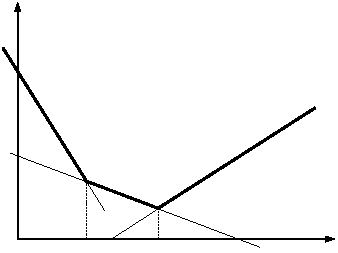
\includegraphics{part_1/chapter_3/figures/Figure2.pdf}};
		\node[right] (1) at (-0.4, 0.4) {$(0,0,1)$};
		\node[right] (2) at (0.4, -0.8) {$(1,1,0)$};	
	\end{tikzpicture}
    \caption{$(0,0,1)$ is degenerate if you add the constraint $x_2 \ge 0$.} \label{p1c3:fig:redundancy_and_degeneration}
\end{figure}


\section{Optimality of extreme points}

Now that we have discussed how to algebraically represent extreme points and have seen a simple mechanism to iterate among their adjacent neighbours, the final element missing for us to be able to devise an optimisation method is to define the optimality conditions we wish to satisfy. In other words, we must define the conditions that, once satisfied, mean that we can stop the algorithm and declare the current solution optimal.


\subsection{The existence of extreme points}

First, let us define the condition that guarantees the existence of extreme points in a polyhedral set. Otherwise, there is no hope of finding an optimal solution.

\begin{definition}[Existence of extreme points]\label{p1c3:def:line_containing}
	A polyhedral set $P \subset \reals^n$ contains a line if $P \neq \emptyset$ and there exists a nonzero vector $d \in \reals^n$ such that $x + \lambda d \in P$ for all $\lambda \in \reals$.
\end{definition}

Figure \ref{p1c3:fig:line_containing} illustrates the notion of containing a line and the existence of extreme points. Notice that if a set would have any ``corner'', then that would imply that a line is contained between the edges that form that corner and, therefore, that corner would be an extreme point.

\begin{figure}[h]
	\begin{tikzpicture}
		\node at (0,0) {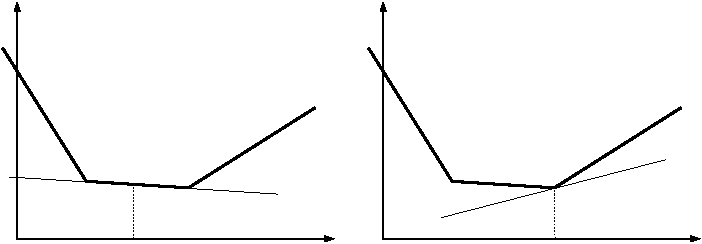
\includegraphics{part_1/chapter_3/figures/Figure3.pdf}};
		\node at (-2.5,0) {$P$};
		\node at (2,-0.3) {$Q$};		
	\end{tikzpicture}
	\caption{$P$ contains a line (left) and $Q$ does not contain a line (right)} \label{p1c3:fig:line_containing}	
\end{figure}

We are now ready to pose the result that utilises Definition \ref{p1c3:def:line_containing} to provide the conditions for the existence of extreme points.

\begin{theorem}[Existence of extreme points]\label{p1c3:thm:exist_extreme_point}
	Let $P = \braces{x \in \reals^n : a_i^\top x \geq b_i, i = 1, \dots, m} \neq \emptyset$ be a polyhedral set. Then the following are equivalent:
	\begin{enumerate}
		\item $P$ has at least one extreme point;
		\item $P$ does not contain a line;
		\item There exists $n$ LI vectors within $\braces{a_i}_{i=1}^m$.	
	\end{enumerate}	
\end{theorem}	 

% TODO: Chp3: add a proof.

It turns out that linear programming problems in the standard form do not contain a line, meaning that they will always provide at least one extreme point (or a basic feasible solution). More generally, bounded polyhedral sets do not contain a line, and neither does the positive orthant.

We are now to state the result that proves the intuition we had when analysing the plots in Chapter \ref{chapter_1}, which states that if a polyhedral set has at least one extreme point and at least one optimal solution, then there must be an optimal solution that is an extreme point.

\begin{theorem}[Optimality of extreme points]\label{p1c3:thm:opt_extreme}
		Let $P = \braces{x \in \reals^n : Ax \geq b}$ be a polyhedral set and $c \in \reals^n$. Consider the problem 
			\begin{equation*}
		    		z = \mini\braces{c^\top x : x \in P}.					
			\end{equation*}
		Suppose that $P$ has at least one extreme point and that there exists an optimal solution. Then, there exists an optimal solution that is an extreme point of $P$.
\end{theorem}

\begin{proof}
	Let $Q = \braces{x \in \reals^n : Ax \geq b, c^\top x = z}$ be the (nonempty) polyhedral set of all optimal solutions. Since $Q \subset P$ and $P$ contains no line (cf. Theorem \ref{p1c3:thm:exist_extreme_point}), $Q$ contains no line either, and thus has an extreme point.

	Let $\overline{x}$ be an extreme point of $Q$. By contradiction, assume that $\overline{x}$ is not an extreme point of $P$. Then, there exist $y \neq \overline{x}$, $w \neq \overline{x}$, and $\lambda \in [0,1]$ such that $\overline{x} = \lambda y + (1-\lambda)w$. Then, $c^\top \overline{x} = \lambda (c^\top y) + (1-\lambda)c^\top w$. As $c^\top \overline{x} = z$ is optimal, we have that $z \leq c^\top y$ and $z \leq c^\top w$,  and thus $z = c^\top y = c^\top w$. 
	
	Thus, $w \in Q$ and $y \in Q$, contradicting that $\overline{x}$ is an extreme point. Thus, $\overline{x}$ must be an extreme point and, since we established that $\overline{x} \in Q$, it is also optimal. 
\end{proof}

Theorem \ref{p1c3:thm:opt_extreme} is posed in a somewhat general way, which might be a source for confusion. First, recall that in the example in Chapter \ref{chapter_1}, we considered the possibility of the objective function level curve associated with the optimal value to be parallel to one of the edges of the feasible region, meaning that instead of a single optimal solution (a vertex), we would observe a line segment containing an infinite number of optimal solutions, of which exactly two would be extreme points. 

In a more general case (with $n > 2$) it might be so that a whole facet of optimal solutions is obtained. That is precisely the polyhedral set of all optimal solutions $Q$ in the proof. Clearly, this polyhedral set will not contain a line and, therefore (cf. Theorem \ref{p1c3:thm:exist_extreme_point}), have at least one extreme point. 

Perhaps another important point is to notice that the result is posed assuming a minimisation problem, but it naturally holds for maximisation problems as well. In fact, maximising a function $f(x)$ is the same as minimising $-f(x)$, with the caveat that, although the optimal value $x^*$ is the same in both cases, the optimal values are symmetric in sign (because of the additional minus we included in the problem being originally maximised).

This is important because we intend to design an algorithm that only inspects extreme points. This discussion guarantees that, even for the cases in which a whole set of optimal solution exists, some elements in that set will be extreme points anyway and thus identifiable by our method.


\subsection{Finding optimal solutions}

We now focus on the issue of being able to find and recognise extreme points as optimal solutions. In general, optimisation methods iterate the following steps:
%
\begin{enumerate}
	\item Start from an initial (often feasible) solution;
	\item Find a nearby solution with better value;
	\item If none are available, return the best-known solution.	
\end{enumerate}
%
This very simple procedure happens to be the core idea of most optimisation methods. We will concentrate on how to identify directions of improvement and, as a consequence of their absence, how to identify optimality.

Starting from a point $x \in P$, we would like to move in a direction $d$ that yields improvement while maintaining feasibility. Definition \ref{p1c3:def:feasible_direction} provides a formalisation of this idea.

\begin{definition}[Feasible directions] \label{p1c3:def:feasible_direction}
	Let $x \in P$, where $P \subset \reals^n$ is a polyhedral set. A vector $d \in \reals^n$ is a feasible direction at $x$ if there exists $\theta > 0$ for which $x + \theta d \in P$.
\end{definition}

Figure \ref{p1c3:fig:feasible_directions} illustrates the concept. Notice that at extreme points, the relevant feasible directions are those along the edges of the polyhedral set since those are the directions that can lead to other extreme points.
  
\begin{figure}[h]
	\begin{tikzpicture}
		\node (0,0) {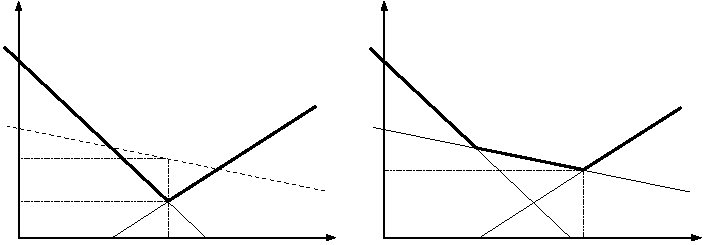
\includegraphics{part_1/chapter_3/figures/Figure4.pdf}};
		\node (P) at (-0.9,0.25) {$P$};
	\end{tikzpicture}
	\caption{Feasible directions at different points of $P$} \label{p1c3:fig:feasible_directions}
\end{figure}

Let us now devise a way of identifying feasible directions algebraically. For that, let $A$ be a $m \times n$ matrix, $I = \braces{1,\dots,m}$ and $J = \braces{1,\dots,n}$. Consider the problem 
%
\begin{equation*}
	\mini \braces{c^\top x : Ax = b, x \geq 0}.	
\end{equation*}
%
Let $x$ be a basic feasible solution (BFS) with basis $B = [A_{B(1)}, \dots, A_{B(m)}]$. Recall that the basic variables $x_B$ are given by
%
\begin{equation*}
	x_B = (x_{B(i)})_{i \in I_B} = B^{-1}b, \text{ with } I_B = \braces{B(1), \dots, B(m)} \subset J,	
\end{equation*}
%
and that the remaining nonbasic variables $x_N$ are such that $x_N = (x_j)_{j \in I_N} = 0$, with $I_N = J \setminus I_B$.

Moving to a neighbouring solution can be achieved by simply moving between adjacent bases, which can be accomplished without significant computational burden. This entails selecting a nonbasic variable $x_j$, $j \in I_N$, and increasing it to a positive value $\theta$. 

Equivalently, we can define a \emph{feasible direction} $d = [d_N, d_B]$, where $d_N$ represent the components associated with nonbasic variables and $d_B$ those associated with basic variables and move from the point $x$ to the point $x + \theta d$. The components $d_N$ associated with the nonbasic variables are thus defined as 
%
\begin{equation*}
d = \begin{cases} d_j = 1 \\ 
				  d_{j'} = 0, \text{for all } j' \neq j, 
	\end{cases}	
\end{equation*}
%
with $j, j' \in I_N$. Notice that, geometrically, we are moving along a line in the dimension represented by the nonbasic variable $x_j$.

Now, feasibility might become an issue if we are not careful to retain feasibility conditions. To retain feasibility, we must observe that $A(x + \theta d) = b$, implying that $Ad = 0$. This allows us to define the components $d_B$ of the direction vector $d$ that is associated with the basic variables $x_j$, $j \in I_B$, since
%
\begin{equation*}
	0 = Ad = \sum_{j = 1}^n	A_j d_j = \sum_{i = 1}^m A_{B(i)}d_{B(i)} + A_j = Bd_B + A_j
\end{equation*}
%
and thus $d_B = -B^{-1} A_j$ is the \emph{basic direction} implied by the choice of the nonbasic variable $x_j$, $j \in I_N$, to become basic. The vector $d_B$ can be thought of as the adjustments that must be made in the value of the other basic variables to accommodate the new variable becoming basic to retain feasibility. 

% TODO: Chp3: this is a complicated concept using a complicated figure.  Rethink this showing a simple example (x_1 + x_2 + x_3 = 1, x_j >= 0) with the "normal feasible region" and the schematic 2d representation. by its side, showing that making 2 out of 3 variables nonbasic yields each of the corners of the triangle. 

Figure \ref{p1c3:fig:adjacent_vertices} provides a schematic representation of this process, showing how the change between adjacent basis can be seen as a movement between adjacent extreme points. Notice that it conveys a schematic representation of a $n=5$ dimensional problem, in which we ignore all the $m$ dimensions and concentrate on the $n-m$ dimensional projection of the feasibility set. This implies that the only constraints left are those associated with the nonnegativity of the variables $x \ge 0$, each associated with an edge of this alternative representation. Thus, when we set $n-m$ (nonbasic variables) to zero, we identify an associated extreme point. As $n-m = 2$, we can plot this alternative representation on $\reals^2$.

\begin{figure}[h]
	\begin{tikzpicture}
		\node (0,0) {\includegraphics{part_1/chapter_3/figures/Figure5.pdf}};
		\node (A) at (-3.2, 1.65) {$A$};
		\node (B) at (-0.2, 1.9) {$B$};
		\node (C) at (3.1, -1.7) {$C$};
		\node[rotate = 90] (x1) at (-3.65, 0) {$x_1 = 0$};
		\node (x2) at (-1.2, -2) {$x_2 = 0$};
		\node (x3) at (-1.9, 1.75) {$x_3 = 0$};
		\node[left] (x4) at (0.25, 0) {$x_4 = 0$};
		\node[right] (x4) at (1.25, 0) {$x_5 = 0$};
	\end{tikzpicture}
	\caption{Example: $n = 5$ and $n-m = 2$. At $A$, $x_1 = x_3 = 0$ and $x_2, x_4, x_5 \geq 0$. Increasing $x_1$ while keeping $x_3$ zero leads to $B$. At $B$, suppose $I_N = \braces{3,5}$; by increasing $x_3$ while keeping $x_5$ zero would leads to $C$.} \label{p1c3:fig:adjacent_vertices}
\end{figure}

Clearly, overall feasibility, i.e., ensuring that $x \ge 0$ can only be retained if $\theta > 0$ is chosen appropriately small. This can be achieved if the following is observed:
%
\begin{enumerate}
	\item All the other nonbasic variables remain valued at zero, that is, $x_{j'} = 0$ for $j' \in I_N \setminus \braces{j}$.	
	\item If $x$ is a \emph{nondegenerate} extreme point, then all $x_B > 0$ and thus $x_B + \theta d_B \geq 0$ for appropriately small $\theta > 0$. 
	\item If $x$ is a \emph{degenerate} extreme point: $d_{B(i)}$ might not be feasible since, for some $B(i)$, if $d_{B(i)} < 0$ and $x_{B(i)} = 0$, any $\theta > 0$ will make $x_{B(i)} < 0$.
\end{enumerate}
%
We will see later that we can devise a simply rule to define a value for $\theta$ that guarantees the above will be always observed. For now, we will put this discussion on hold and focus on the issue of how to guide the choice of which nonbasic variable $x_j$, $j \in I_N$, to select to become basic.


\subsection{Moving towards improved solutions}

A simple yet efficient way of deciding which nonbasic component $j \in I_N$ to make basic is to consider the immediate potential benefit that it would have for the objective function value. 

Using objective function $c^\top x$, if we move along the feasible direction $d$ as previously defined, we have that the objective function value changes by 
%
\begin{equation*}
	c^\top d = c_B^\top d_B + c_j = c_j - c_B^\top B^{-1}A_j,
\end{equation*}
%
where $c_B = [c_{B(1)}, \dots, c_{B(m)}]$. The quantity $c_j - c_BB^{-1}A_j$ can be used, for example, in a greedy fashion, meaning that we choose the nonbasic variable index $j \in I_N$ with greatest \emph{potential of improvement}.

First, let us formally define this quantity, which is known as the \emph{reduced cost}. 

\begin{definition}[Reduced cost]
	Let $x$ be a basic solution associated with the basis $B$ and let $c_B = [c_{B(1)}, \dots, c_{B(m)}]$ be the objective function coefficients associated with the basis $B$. For each nonbasic variable $x_j$, with $j \in I_N$, we define the reduced cost $\overline{c}_j$ as
	%
	\begin{equation*}
		\overline{c}_j = c_j - c_B^\top B^{-1}A_j.
	\end{equation*}
\end{definition}

The name reduced cost is motivated by the fact that it quantifies a cost change onto the reduced space of the basic variables. In fact, the reduced cost is calculating the change in the objective function caused by the increase in one unit of the nonbasic variable $x_j$ elected to become basic (represented by the $c_j$ component) and the associated change caused by the accommodation in the basic variable values to retain feasibility, as discussed in the previous section. Therefore, the reduced cost can be understood as a \emph{marginal value} of change in the objective function value associated with each nonbasic variable.

Let us demonstrate this with a numerical example. Consider the following linear programming problem
%
\begin{align*}
	\mini & 2x_1 + 1x_2 + 3x_3 + 2x_4 \\	
	\st & x_1 + x_2 + x_3 + x_4 = 2 \\
	& 2x_1 + 3x_3 + 4x_4 = 2 \\
	& x_1, x_2 ,x_3, x_4 \geq 0.  
\end{align*}  
%
Let $I_B = \braces{1,2}$, yielding
% 
\begin{equation*}
	B = \begin{bmatrix}
    		1 & 1 \\
    		2 & 0
    	\end{bmatrix}.
\end{equation*} 
%
Thus, $x_3= x_4 =0$ and $x = (1,1,0,0)$. The basic direction $d_B^3$ for $x_3$ is given by
%
\begin{equation*}
    d_B^3 = -B^{-1}A_3 = -\begin{bmatrix}
    	0 & 1/2 \\
    	1 & -1/2
    \end{bmatrix} \begin{bmatrix}
    	1 \\ 3
    \end{bmatrix} = \begin{bmatrix}
    	-3/2 \\ 1/2
    \end{bmatrix}.
\end{equation*}
%
which gives $d^3 = (-3/2, 1/2, 1, 0)$. Analogously, for $x_4$, we have
%
\begin{equation*}
    d_B^4 = -B^{-1}A_4 = -\begin{bmatrix}
    	0 & 1/2 \\
    	1 & -1/2
    \end{bmatrix} \begin{bmatrix}
    	1 \\ 4
    \end{bmatrix} = \begin{bmatrix}
    	-2 \\ 1
    \end{bmatrix}.
\end{equation*}


The (reduced) cost of moving along the direction given by $d^3$ is 
%
\begin{equation*}
	c^\top d^3 = (c_1, c_2)^\top d_B^3 + c_3 = ((-3/2)2 + (1/2)1) + 3 = 0.5
\end{equation*}
%
while moving along $d^4$ has a cost of
\begin{equation*}
	c^\top d^4 = (c_1, c_2)^\top d_B^4 + c_4 = ((-2)2 + (1)1) + 2 = -1.
\end{equation*}
%
Thus, between $d^3$ and $d^4$, $d^4$ is a better direction since its reduced cost indicates a reduction of $1$ unit of the objective function per unit of $x_4$. In contrast, the reduced cost associated with $d^3$ indicates an increase of 0.5 units of the objective function per unit of $x_3$, indicating that this is a direction to be avoided as we are minimising the problem.
%
Clearly, the willingness to choose $x_{j'}$, $j' \in I_N$ as the variable to become basic will depend on whether the scalar $c_{j'} - (c_j)_{j \in I_B}^\top d_B$ is negative (recall that we want to minimise the problem, so the smaller the total cost, the better). Another point is how large in module the reduced cost is. Recall that the reduced cost is, in fact, a measure of the marginal value associated with the increase in value of the nonbasic variable. Thus the more negative it is, the quicker the objective function value will decrease per unit of increase of the nonbasic variable value.
%
One interesting thing to notice is what is the reduced cost associated with basic variables. Recall that $B = [A_{B(1)}, \dots, A_{B(m)}]$ and thus $B^{-1}[A_{B(1)}, \dots, A_{B(m)}] = I$. Therefore $B^{-1}A_{B(i)}$ is the $i^\text{th}$ column of $I$, denoted $e_i$, implying that
%
\begin{equation*}
	\overline{c}_{B(i)} = c_{B(i)} - c^\top_B B^{-1} A_{B(i)} = c_{B(i)} - c_B^\top e_i = c_{B(i)} - c_{B(i)} = 0.	
\end{equation*}


\subsection{Optimality conditions}

Now that we have seen how to identify promising directions for improvement, we have incidentally developed a framework for identifying the optimality of a given basic feasible solution (BFS). That is, a BFS from which no direction of improvement can be found must be locally optimal. And, since local optimality implies global optimality in the presence of convexity (the convexity of linear programming problems was attested in Chapter \ref{chapter_2}; the global optimality in the presence of convexity is a result discussed in detail in Part \ref{part_2}), we can declare this BFS as an optimal solution. 

%TODO: Chp3: connect this with the new result of convexity removed from HW2 

Theorem \ref{p1c3:thm:opt_conditions} establishes the optimality of a BFS from which no improving feasible direction can be found without explicitly relying on the notion of convexity.

\begin{theorem}[Optimality conditions]\label{p1c3:thm:opt_conditions}
	Consider the problem $P : \mini\braces{c^\top x : Ax = b, x \geq 0}$. Let $x$ be the BFS associated with a basis $B$ and let $\overline{c}$ be the corresponding vector of reduced costs.
	\begin{enumerate}
		\item[(1)] if $\overline{c} \geq 0$, then $x$ is optimal.
		\item[(2)] if $x$ is optimal and nondegenerate, then $\overline{c} \geq 0$.	
	\end{enumerate}
\end{theorem}

\begin{proof}
To prove (1), assume that $\overline{c}_j \geq 0$, let $y$ be a feasible solution to $P$, and $d = y - x$. We have that $Ax = Ay = b$ and thus $Ad = 0$. Equivalently:
%
\begin{align}
	&B d_B + \sum_{j \in I_N}A_j d_j = 0 \Rightarrow d_B = - \sum_{j \in I_N}B^{-1}A_jd_j, \text{ implying that } \nonumber \\
	&c^\top d = c_B^\top d_B + \sum_{j \in I_N}c_jd_j= \sum_{j \in I_N} (c_j - c_B^\top B^{-1}A_j)d_j = \sum_{j \in I_N}\overline{c}_jd_j \label{p1c3:eq:red_cost_opt_cond}
\end{align}
%
We have that $x_j = 0$ and $y_j \geq 0$	for $j \in I_N$. Thus, $d_j \geq 0$ and $\overline{c}_jd_j \geq 0$ for $j \in I_N$, which implies that $c^\top d \geq 0$ (cf. \eqref{p1c3:eq:red_cost_opt_cond}). Consequently,
%
\begin{equation*}
	c^\top d \geq 0 \Rightarrow	c^\top (y - x) \geq 0 \Rightarrow c^\top y \geq c^\top x, \text{ i.e., $x$ is optimal.}
\end{equation*}
%
To prove (2) by contradiction, assume that $x$ is optimal with $\overline{c}_j < 0$ for some $j \in I_N$. Thus, we could improve on $x$ moving along this $j^\text{th}$ direction $d$, contradicting the optimality of $x$.
\end{proof}

A couple of remarks are worth making at this point. First, notice that, in the presence of degeneracy, it might be that $x$ is optimal with $\overline{c}_j < 0$ for some $j \in I_N$. Luckily, the simplex method manages to get around this issue in an effective manner, as we will see in the next chapter. Another point to notice is that, if $\overline{c}_j > 0$, $\forall j \in I_N$, then $x$ is a \emph{unique optimal}. Analogously, if $\overline{c} \geq 0$ with $c_j =0$ for some $j \in I_N$, then it means that moving in that direction will cause no change in the objective function value, implying that both BFS are ``equally optimal'' and that the problem has multiple optimal solutions. 

\vfill
\pagebreak
\section{Exercises}

\subsection*{Exercise 3.1: Properties of basic solutions}

Prove the following theorem:

\begin{theorem*}[Linear independence and basic solutions] 
	\small
	Consider the constraints $Ax = b$ and $x \geq 0$, and assume that $A$ has $m$ LI rows $M = \braces{1,\dots,m}$. A vector $\overline{x} \in \reals^n$ is a \emph{basic solution} if and only if we have that $A\overline{x} = b$ and there exists indices $B(1), \dots, B(m)$ such that
	\begin{enumerate}
		\item The columns $A_{B(1)}, \dots, A_{B(m)}$ are LI
		\item If $j \neq B(1), \dots, B(m)$, then $\overline{x}_j = 0$.
	\end{enumerate} 
\end{theorem*}

Note: the theorem is proved in the notes. Use this as an opportunity to revisit the proof carefully, and try to take as many steps without consulting the text as you can. This is a great exercise to help you internalise the proof and its importance in the context of the material. I strongly advise against blindly memorising it, as I suspect you will never (in my courses, at least) be requested to recite the proof literally.

\subsection*{Exercise 3.2: Basic solutions and extreme points}

Consider the set $P=\{\mathbf{x}\in\mathbb{R}^2 : x_1 + x_2 \leq 6,~ x_2 \leq 3,~ x_1, x_2 \geq0\}$. 

\begin{itemize}
\item[(a)] Enumerate all basic solutions, and identify those that are basic feasible solutions.
\item[(b)] Draw the feasible region, and identify the extreme point associated with each basic feasible solution.
\item[(c)] Consider a minimization problem with the cost vector $\mathbf{c'}=(c_1,c_2,c_3,c_4)=(-2,\frac{1}{2},0,0)$. Compute the basic directions and the corresponding reduced costs of the nonbasic variables at the basic solution $\mathbf{x'}=(3,3,0,0)$ with $\mathbf{x}'_B=(x_1,x_2)$ and $\mathbf{x}'_N=(x_3,x_4)$; either verify that $\mathbf{x'}$ is optimal, or move along a basic direction which leads to a better solution. 
\end{itemize}

\subsection*{Exercise 3.3: Degeneracy - part 1}

Given the linear program given below,

\begin{center}
	\begin{enumerate}
		\begin{tabular}{*4c}
			$\max$ & $2x_1 + x_2$ & \\
			s.t. \\
			& $2x_1 + 2x_2$ & $\leq$ & $9$  \\
			& $2x_1 -  x_2$ & $\leq$ & $3$   \\
			& $ x_1 -  x_2$ & $\leq$ & $1$   \\
			& $4x_1 - 3x_2$ & $\leq$ & $5$   \\
			& $x_1$         & $\leq$ & $2.5$ \\
			& $x_2$         & $\leq$ & $4$   \\
			\\
			\multicolumn{4}{c}{$x_1, x_2 \geq 0$}\\
		\end{tabular}
	\end{enumerate}
\end{center}

\begin{itemize}
	\item[(a)] Plot the constraints and find the degenerate basic feasible solutions.
	\item[(b)] What are the bases forming the degenerate solutions?
\end{itemize}

\subsection*{Exercise 3.4: Feasible direction}

Let $x$ be a point in a polyhedron $P=\braces{x \in \reals^n : Ax =  b, x \ge 0}$. Show that a vector $d \in \reals^n$ is a feasible direction at $x \in P$ if and only if $ Ad = 0$ and $d_i\ge 0$ for all $i$ for which $x_i = 0$.  A feasible direction of $P$ at point $x$ is a vector $d \neq 0$ such that $x + \theta d \in P$ for some $\theta > 0$.


\subsection*{Exercise 3.5: Optimality of extreme points}

Prove the following theorem.

\begin{theorem*}[Optimality of extreme points] 
	\small
	Let $P = \braces{x \in \reals^n : Ax \geq b}$ be a polyhedral set and $c \in \reals^n$. Consider the problem 
	\begin{equation*}
		z = \mini\braces{c^\top x : x \in P}.					
	\end{equation*}
	Suppose that $P$ has at least one extreme point and that there exists an optimal solution. Then, there exists an optimal solution that is an extreme point of $P$.
\end{theorem*}

Note: see Exercise 3.1.





